\begin{figure*}[t]
\centering
% Vector drawing generated by tools/figures/example.py; rerun it after changing the figure.
\ifbilingual
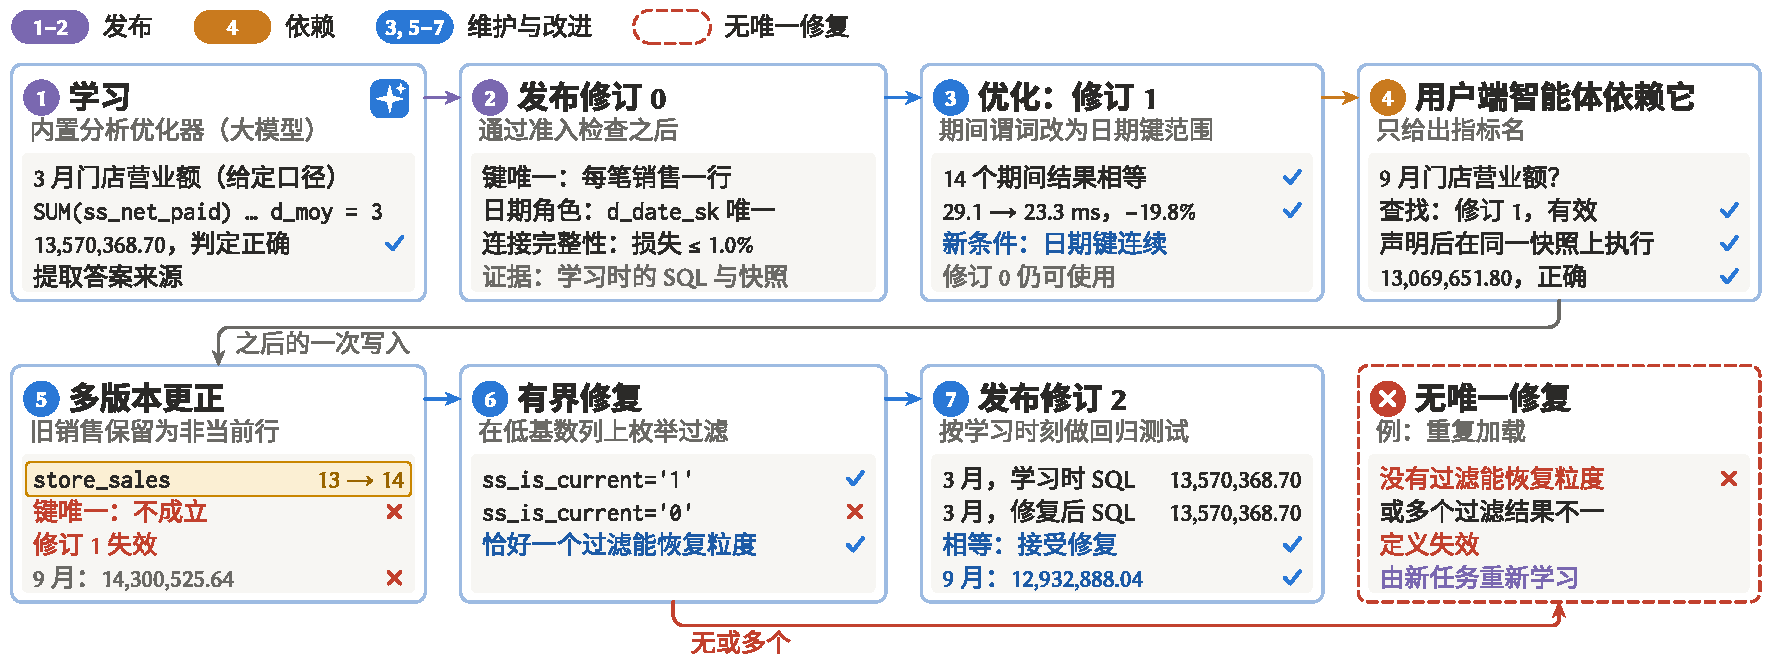
\includegraphics[width=\textwidth]{figures/running-example-zh}
\else
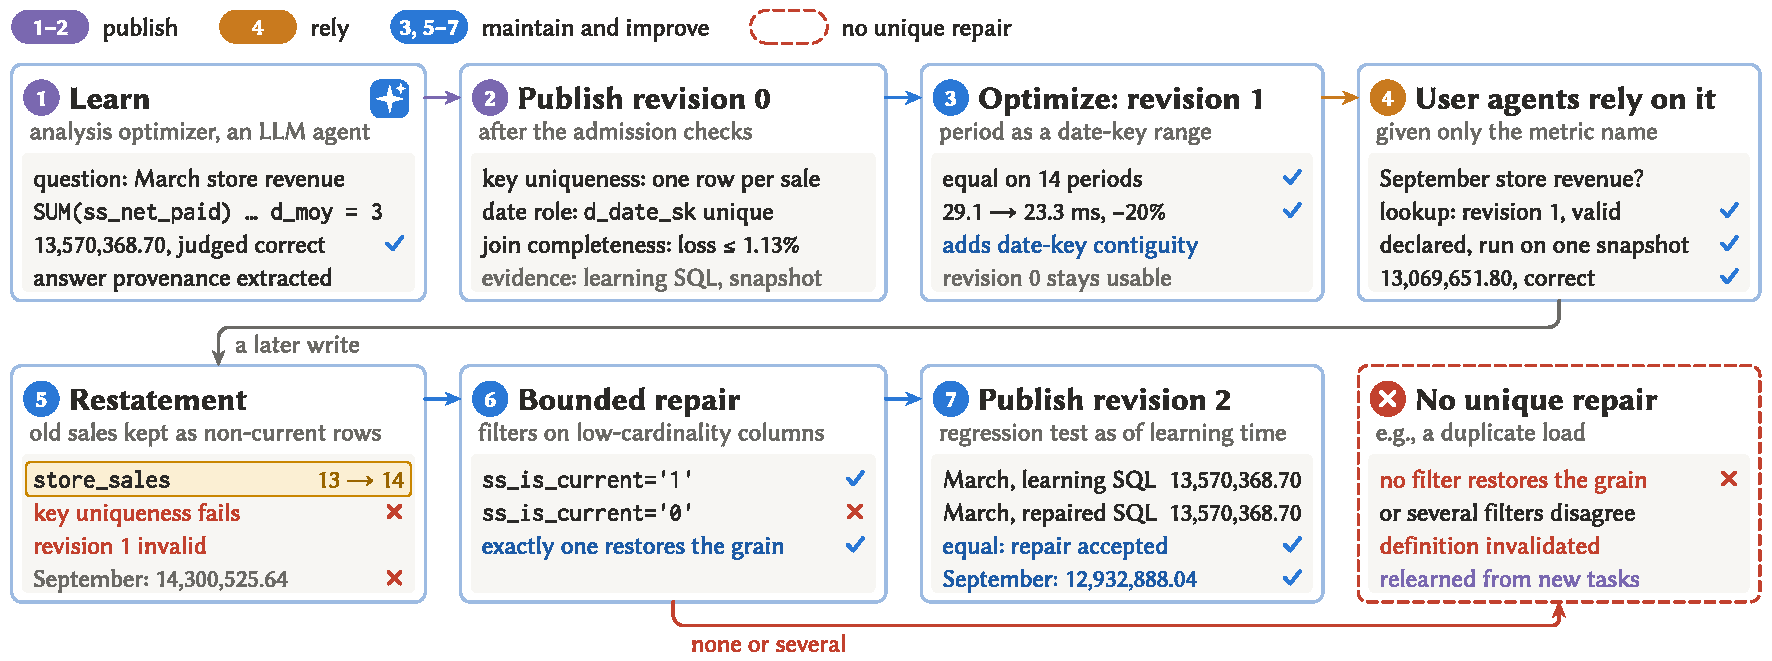
\includegraphics[width=\textwidth]{figures/running-example}
\fi
\caption{\bt{One shared definition, store revenue, in \system\ (values recorded on one million sales rows). Publish (1--2): the judged answer of the analysis optimizer becomes revision~0, with conditions derived from its structure. Improve (3): an equivalent key-range rewrite is 19.8\% faster and becomes revision~1, which adds date-key contiguity as a maintained condition. Rely (4): user agents that know only the metric name use the valid revision on their snapshot. Maintain (5--7): a restatement raises the version of \code{store\_sales} and breaks key uniqueness, so revision~1 is invalid; the one filter that restores the grain and reproduces the learning answer as of learning time becomes revision~2. Used as written, revision~1 would return 14,300,525.64 for September.}{\system\ 中的一个共享定义：门店营业额（数值记录自 100 万行销售数据）。发布（1--2）：分析优化器判定正确的答案成为修订 0，条件由其结构推出。改进（3）：等价的日期键范围改写快 19.8\%，成为修订 1，并新增日期键连续这一受维护的条件。依赖（4）：只知道指标名的用户端智能体在自己的快照上使用有效修订。维护（5--7）：多版本更正使 \code{store\_sales} 的版本升高并破坏键唯一性，修订 1 失效；唯一能恢复粒度、并按学习时刻复现学习答案的过滤成为修订 2。若照原样执行修订 1，9 月将返回 14,300,525.64。}}
\label{fig:example}
\Description{Eight boxes in two rows. Top row: (1) Learn: the analysis optimizer, an LLM agent, answers March store revenue with SUM(ss_net_paid), 13,570,368.70, judged correct; (2) Publish revision 0 after the admission checks, with key uniqueness, date role, join completeness, and evidence; (3) Optimize: revision 1 expresses the period as a date-key range, equal on 14 periods, 29.1 to 23.3 ms, adding date-key contiguity; (4) User agents rely on it: a lookup returns revision 1, the declared query runs on one snapshot, 13,069,651.80, correct. An arrow labelled "a later write" leads to the bottom row: (5) Restatement: store_sales version 13 to 14, key uniqueness fails, revision 1 invalid, September as written 14,300,525.64; (6) Bounded repair: ss_is_current='1' passes, ss_is_current='0' fails, exactly one filter restores the grain; (7) Publish revision 2 after a regression test as of learning time: March with the learning SQL and the repaired SQL both 13,570,368.70, September 12,932,888.04. A red dashed box, reached when none or several filters work, shows the other outcome: no unique repair, e.g. after a duplicate load, the definition is invalidated and relearned.}
\end{figure*}
